\chapter{等角写像と開弦散乱の処方}

\lectureoverview{等角写像は、まず二次元静電場の実用的な対称性として現れる。複素微分可能性がその対称性を計算可能なものに変える。すなわち、Cauchy--Riemann方程式はLaplace方程式を導き、方向に依存しない複素導関数は角度を保つ。この道具立てを手にすると、弦の世界面は物理を変えることなく、帯、半平面、円柱、または円板として描くことができる。すると開弦散乱は、その境界上に運動量挿入を持つ円板上のGauss経路積分となり、続いてそれらの非等価な位置に関する積分となる。}

\section{二次元世界における静電場}

文字通りの二次元静電場の問題から始める。電荷とその場の線は平面に閉じ込められており、単に運動がたまたま平面的であるような通常の三次元電荷ではない。するとGaussの法則は次を与える。
\begin{equation}
  F(r)\propto \frac{1}{r},
  \qquad
  V(r)\propto \log r,
  \label{eq:l08-two-dimensional-coulomb}
\end{equation}
なぜなら、流束は円周が\(r\)のように増大する円を横切るからである。

場をスカラー・ポテンシャル\(\phi\)で表す。黒板で用いた符号の規約では、
\begin{equation}
  \mathbf E=\nabla\phi,
  \qquad
  \nabla\cdot\mathbf E=\rho,
\end{equation}
であり、したがって
\begin{equation}
  \nabla^2\phi
  =\frac{\partial^2\phi}{\partial x^2}
  +\frac{\partial^2\phi}{\partial y^2}
  =\rho.
  \label{eq:l08-poisson}
\end{equation}
である。電荷のない領域では、これはLaplace方程式に帰着する。
\begin{equation}
  \nabla^2\phi=0.
  \label{eq:l08-laplace-phi}
\end{equation}
\editorialnote{多くの電気力学の教科書は
\(\mathbf E=-\nabla\Phi\)と定義し、その場合、定数を吸収した後で
\(\nabla^2\Phi=-\rho\)となる。この講義では反対のポテンシャル符号を用いる。源のない方程式とすべての等角論法は変わらない。}

\begin{figure}[H]
  \centering
  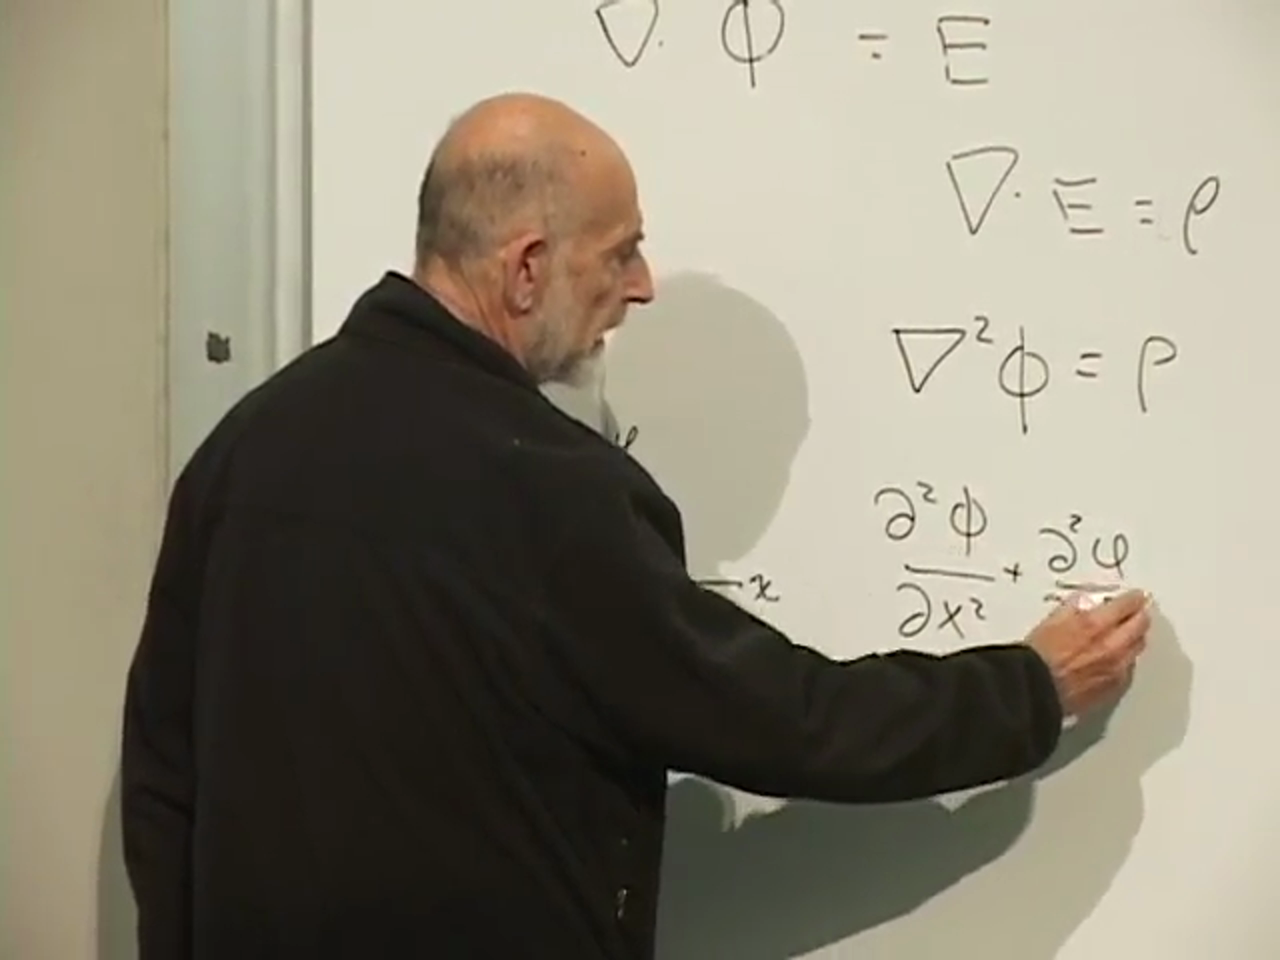
\includegraphics[width=0.72\textwidth]{lecture_08_figure_01.png}
  \caption{静電場の方程式を二次元Poisson演算子へと展開したもの。}
  \lectureframe{00:03:48}
  \label{fig:l08-electrostatics-board}
\end{figure}

二つの空間微分の間のプラス符号が重要である。これにより、これが波動方程式ではなく楕円型方程式となる。等角変換はその源のない形を保つので、ある領域上の解はその境界条件とともに、異なる形の領域へ移すことができる。これは弦理論で役立つ前に、静電場、二次元流体の流れ、および地図作成において役立つ。

\begin{classroomqa}
\audiencequestion{Laplacianがゼロなら、これは定在波方程式か？ \lecturetimestamp{00:05:35}}
\lecturerresponse{いいえ。二つの空間微分は同じ符号を持ち、時間微分はない。波動方程式には、Lorentz的な相対符号を伴う時間依存性が必要である。静電場が静的であるのは、波を含め何も発展していないからまさにである。}
\end{classroomqa}

\begin{classroomqa}
\audiencequestion{二次元に回転はあるか？
\lecturetimestamp{00:06:06}}
\lecturerresponse{あるが、独立な成分は一つだけである。
\(\mathbf E=(E_x,E_y)\)に対して、
\[
  \operatorname{curl}_{2d}\mathbf E
  =\partial_yE_x-\partial_xE_y.
\]
これは黒板に垂直な成分として描いてもよいが、本質的に二次元の世界には外部の垂直方向は必要ない。より高次元では、対応する対象は自然に反対称二形式である。}
\end{classroomqa}

\section{優先方向を持たない導関数}

元の平面と像平面に複素座標を導入する。
\begin{equation}
  z=x+iy,
  \qquad
  w=u+iv,
  \qquad
  w=w(z).
  \label{eq:l08-complex-coordinates}
\end{equation}
ここで\(x,y,u,v\)は実数である。局所的には、導関数は
\begin{equation}
  \frac{dw}{dz}
  =\lim_{\Delta z\to0}\frac{\Delta w}{\Delta z}.
  \label{eq:l08-complex-derivative}
\end{equation}
であるべきである。複素平面は実数直線と異なり、無限に多くの接近方向を許す。連続で通常の意味で滑らかな写像は、各方向に沿って同じ比を与える必要はない。

二つの簡単な接近法を比較する。\(x\)方向に沿っては\(dy=0\)なので、
\begin{equation}
  \left.\frac{dw}{dz}\right|_x
  =\frac{\partial u}{\partial x}
  +i\frac{\partial v}{\partial x}.
\end{equation}
である。\(y\)方向に沿っては\(dx=0\)であり、
\begin{equation}
  \left.\frac{dw}{dz}\right|_y
  =\frac{1}{i}\frac{\partial u}{\partial y}
  +\frac{\partial v}{\partial y}
  =\frac{\partial v}{\partial y}
  -i\frac{\partial u}{\partial y}.
\end{equation}
である。実部と虚部の等置から
\begin{equation}
  \boxed{
  \frac{\partial u}{\partial x}
  =\frac{\partial v}{\partial y},
  \qquad
  \frac{\partial u}{\partial y}
  =-\frac{\partial v}{\partial x}}
  \label{eq:l08-cauchy-riemann}
\end{equation}
が得られる。これらがCauchy--Riemann方程式である。通常の微分可能性の仮定の下では、それらは極限
\eqref{eq:l08-complex-derivative}が方向に依存しないための十分条件でもある。この性質を持つ関数は、その点で解析的、すなわち正則である。

\begin{figure}[H]
  \centering
  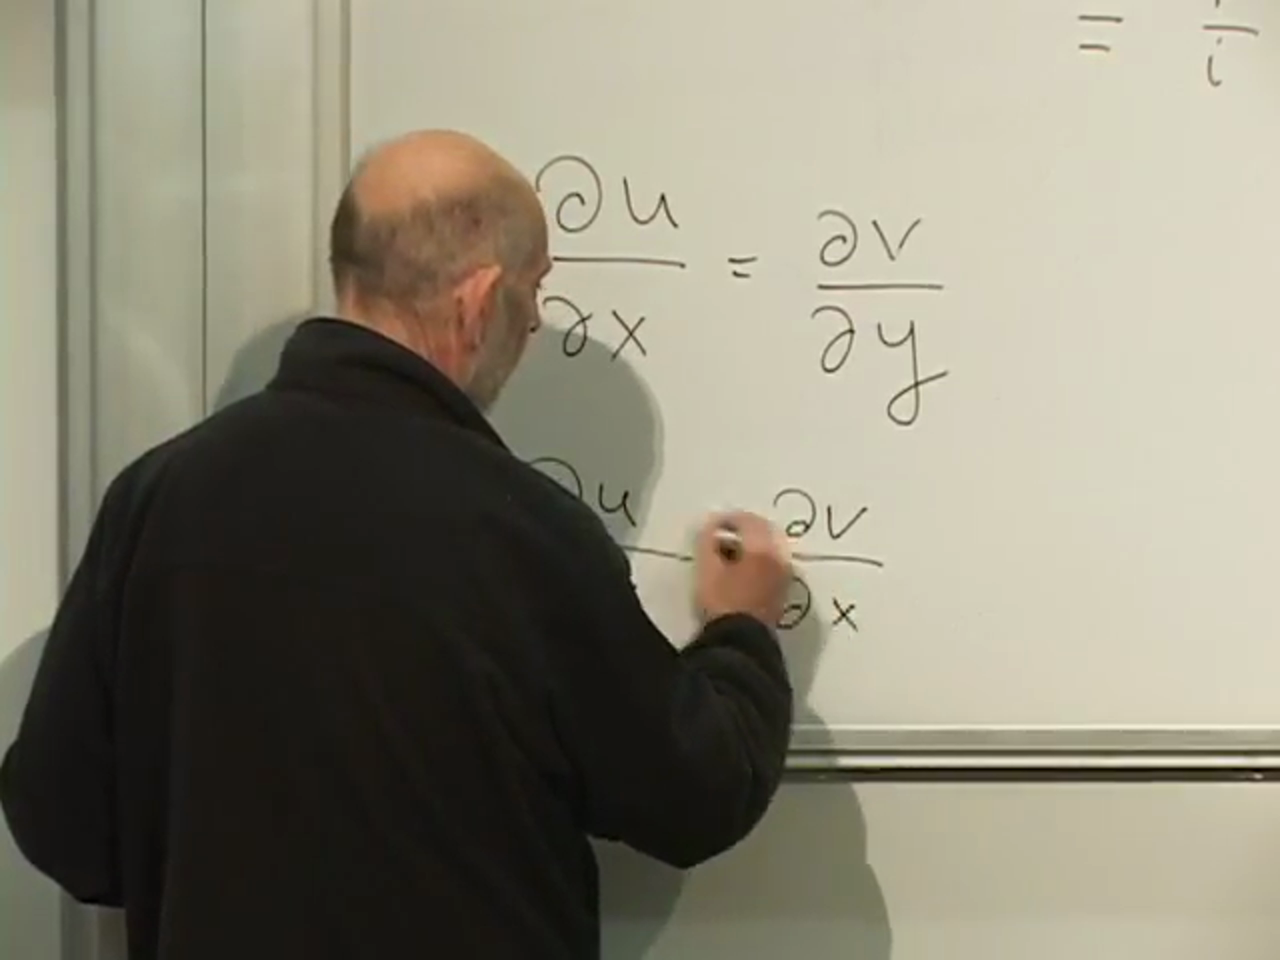
\includegraphics[width=0.70\textwidth]{lecture_08_figure_02.png}
  \caption{相対的なマイナス符号を含む、完成したCauchy--Riemannの組。}
  \lectureframe{00:19:48}
  \label{fig:l08-cr-board}
\end{figure}

講義では関連する用語を簡単に区別する。有限な複素平面全体で正則な関数は整関数である。有理型関数は孤立した極を持ちうる。したがって\(1/z\)は\(z=0\)から離れたところで解析的であるが、整関数ではない。

\section{調和共役と等角幾何}

コーシー--リーマンの方程式は連立一階方程式であるが、それらは分離された二階方程式を導く。\(\partial_xu=\partial_yv\)を\(x\)で微分し、\(\partial_yu=-\partial_xv\)を\(y\)で微分して加えると、
\begin{align}
  \partial_x^2u&=\partial_x\partial_yv,\\
  \partial_y^2u&=-\partial_y\partial_xv,\\
  \therefore\qquad
  \partial_x^2u+\partial_y^2u&=0.
  \label{eq:l08-harmonic-u}
\end{align}
\(u\)と\(v\)を入れ替えて同じ議論を繰り返すと、
\begin{equation}
  \partial_x^2v+\partial_y^2v=0.
  \label{eq:l08-harmonic-v}
\end{equation}
が得られる。したがって、解析関数の実部と虚部は調和共役である。任意の二つの調和関数が自動的に解析関数を作るわけではなく、それらは依然として\eqref{eq:l08-cauchy-riemann}によって結び付けられていなければならない。

\begin{figure}[H]
  \centering
  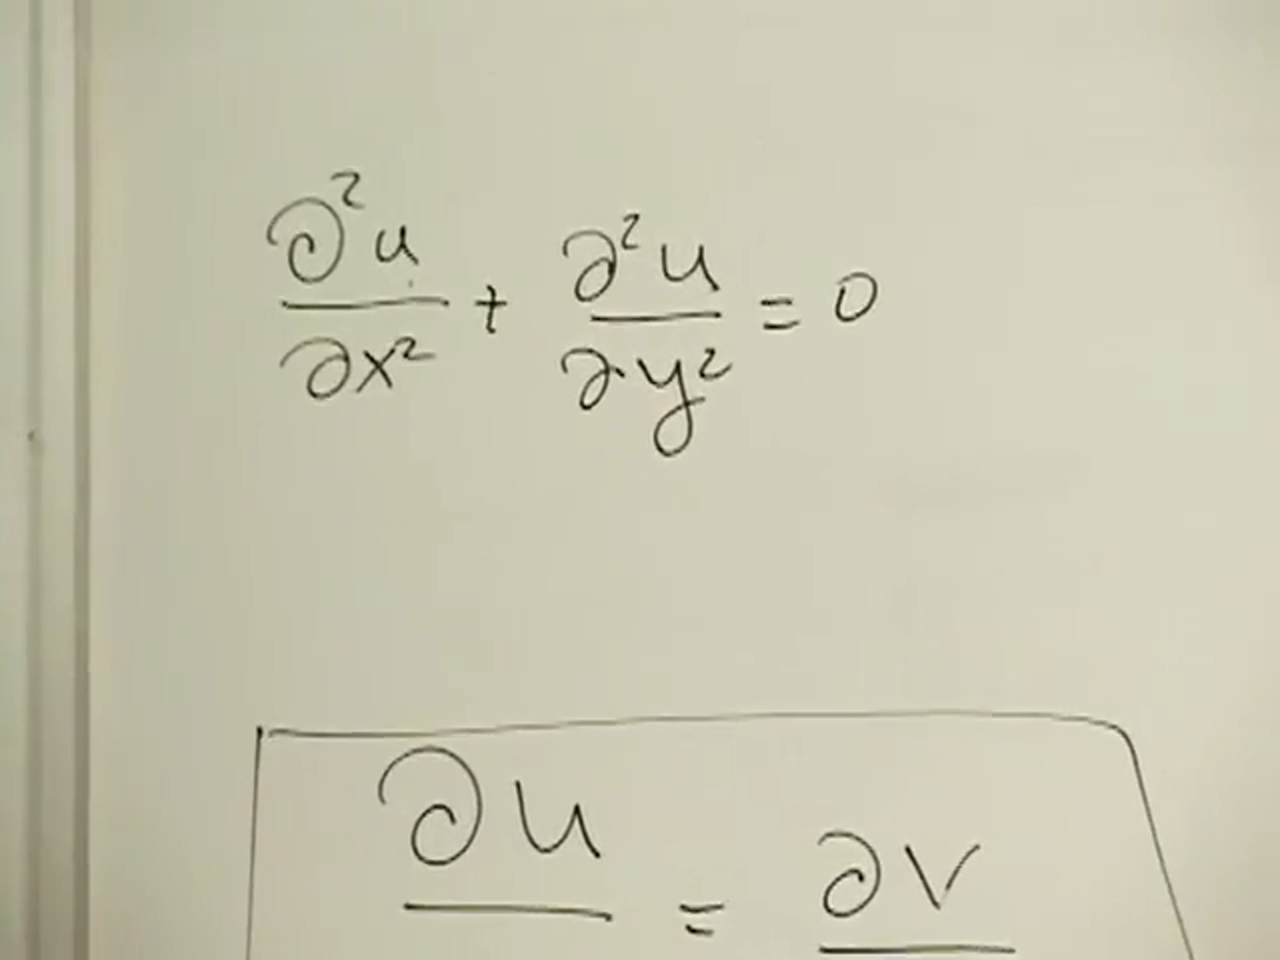
\includegraphics[width=0.68\textwidth]{lecture_08_figure_03.png}
  \caption{混合導関数が相殺し、解析写像の一つの成分に対するラプラス方程式が残る。}
  \lectureframe{00:23:09}
  \label{fig:l08-harmonic-board}
\end{figure}

有用なベクトル的解釈もある。\(\mathbf F=(u,-v)\)とすると、二つのコーシー--リーマンの方程式は、選んだ向きの規約の範囲内で、\(\mathbf F\)の発散と二次元回転の両方が消えることを述べている。これが約束した静電学への回帰である。

\subsection{なぜ角度が保たれるのか}

二つの微小な複素変位を極形式で書く：
\begin{equation}
  \delta z=\rho e^{i\theta},
  \qquad
  \Delta z=\rho'e^{i\theta'}.
\end{equation}
それらの比の位相は\(\theta-\theta'\)であり、まさにそれらの間の角度である。解析写像の下で、
\begin{equation}
  \frac{\delta w}{\delta z}
  =\frac{\Delta w}{\Delta z}
  =w'(z),
\end{equation}
なぜなら導関数は方向に依存しないからである。整理すると、
\begin{equation}
  \frac{\Delta z}{\delta z}
  =\frac{\Delta w}{\delta w}.
  \label{eq:l08-angle-ratio}
\end{equation}
両辺は同じ位相をもつので、元の区間の間の角度はそれらの像の間の角度に等しい。

\begin{figure}[H]
  \centering
  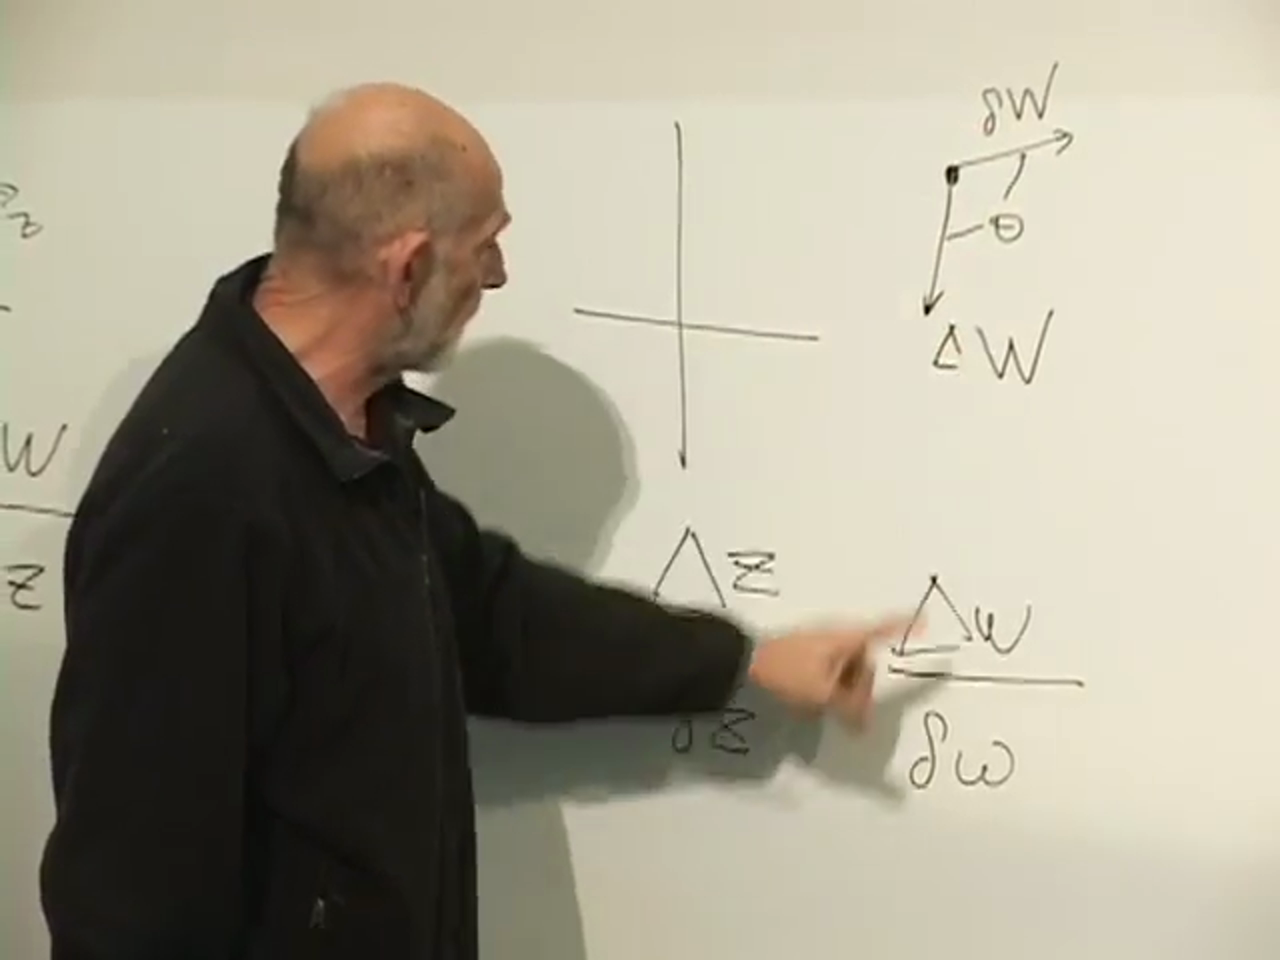
\includegraphics[width=0.70\textwidth]{lecture_08_figure_04.png}
  \medskip

  \begin{tikzpicture}[x=0.9cm,y=0.9cm,>=Latex]
    \begin{scope}
      \draw[->] (-0.2,0) -- (2.3,0);
      \draw[->] (0,-0.2) -- (0,2.1);
      \draw[very thick,blue!65!black,->] (0,0) -- (1.85,0.45)
        node[right] {\(\delta z\)};
      \draw[very thick,orange!75!black,->] (0,0) -- (0.72,1.65)
        node[above] {\(\Delta z\)};
      \draw (0.58,0.14) arc[start angle=14,end angle=66,radius=0.60];
      \node at (1.0,-0.55) {\(z\)-plane};
    \end{scope}
    \draw[->,thick] (3.0,0.9) -- (4.2,0.9)
      node[midway,above] {\(w(z)\)};
    \begin{scope}[xshift=5.0cm]
      \draw[->] (-0.2,0) -- (2.3,0);
      \draw[->] (0,-0.2) -- (0,2.1);
      \draw[very thick,blue!65!black,->] (0,0) -- (1.65,0.70)
        node[right] {\(\delta w\)};
      \draw[very thick,orange!75!black,->] (0,0) -- (0.48,1.62)
        node[above] {\(\Delta w\)};
      \draw (0.54,0.23) arc[start angle=23,end angle=74,radius=0.59];
      \node at (1.0,-0.55) {\(w\)-plane};
    \end{scope}
  \end{tikzpicture}
  \caption{黒板での証明と簡潔な局所的再構成。\(w'(z)\)による乗算は、あらゆる無限小方向を同じ量だけ回転させ、拡大縮小し、それらの相対角度を保つ。}
  \lectureframe{00:34:11}
  \label{fig:l08-angle-proof}
\end{figure}

この局所的議論は\(w'(z)\neq0\)を仮定している。臨界点では写像は局所的に一対一でない可能性があり、幾何学を別途扱わなければならない。そのような点から離れては、解析写像と向きを保つ等角写像は局所的に同じ対象である。

\section{目を養う例}

\subsection{二乗と複素共役}

\(w=z^2\)に対して、
\begin{equation}
  (x+iy)^2=x^2-y^2+2ixy=u+iv,
\end{equation}
したがって
\begin{equation}
  u=x^2-y^2,
  \qquad
  v=2xy.
  \label{eq:l08-z-squared-components}
\end{equation}
\(u\)の二階導関数は\(2\)と\(-2\)であり、\(v\)のそれらは別々に消える。両方とも調和であり、直接微分することによりコーシー--リーマンの方程式も確認できる。

\begin{figure}[H]
  \centering
  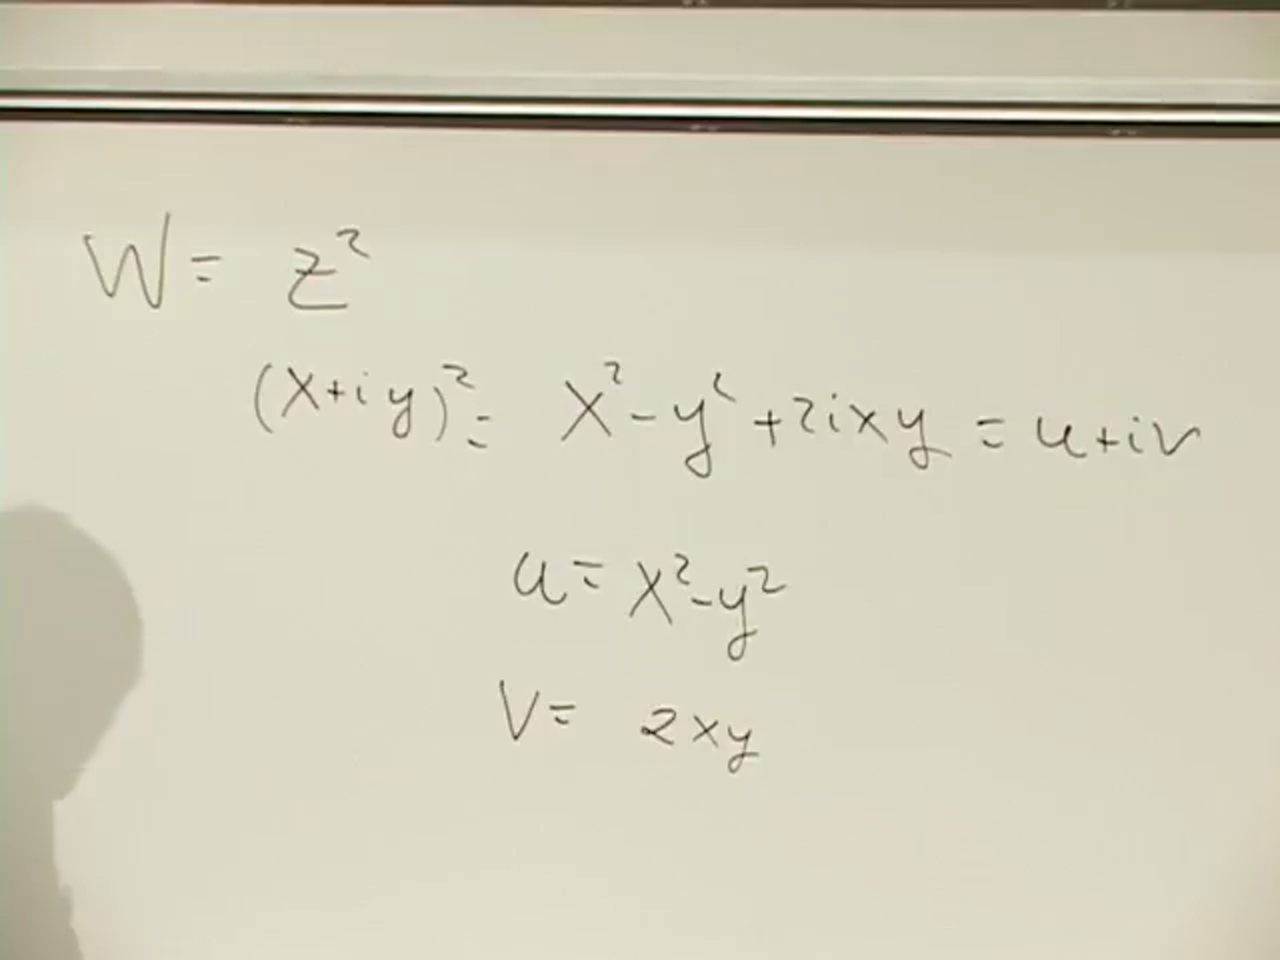
\includegraphics[width=0.72\textwidth]{lecture_08_figure_05.png}
  \caption{二乗写像をその実部と虚部の調和成分に分けたもの。}
  \lectureframe{00:36:45}
  \label{fig:l08-z-square-board}
\end{figure}

\begin{classroomqa}
\audiencequestion{\(1/z\)は非解析的な例を与えるか？
\lecturetimestamp{00:37:49}}
\lecturerresponse{一点でのみである。\(z\neq0\)であるところではどこでも解析的であり、原点に極をもつ。至る所でコーシー--リーマンの判定に失敗する写像を見るには、複素共役の方がより良い例である。}
\end{classroomqa}

対照的に、
\begin{equation}
  w=\bar z=x-iy
  \qquad\Longrightarrow\qquad
  u=x,\quad v=-y
\end{equation}
は向きを逆転させる。その導関数は符号によって第一のコーシー--リーマンの方程式に失敗するので、\(z\)の関数として解析的ではない。

\begin{figure}[H]
  \centering
  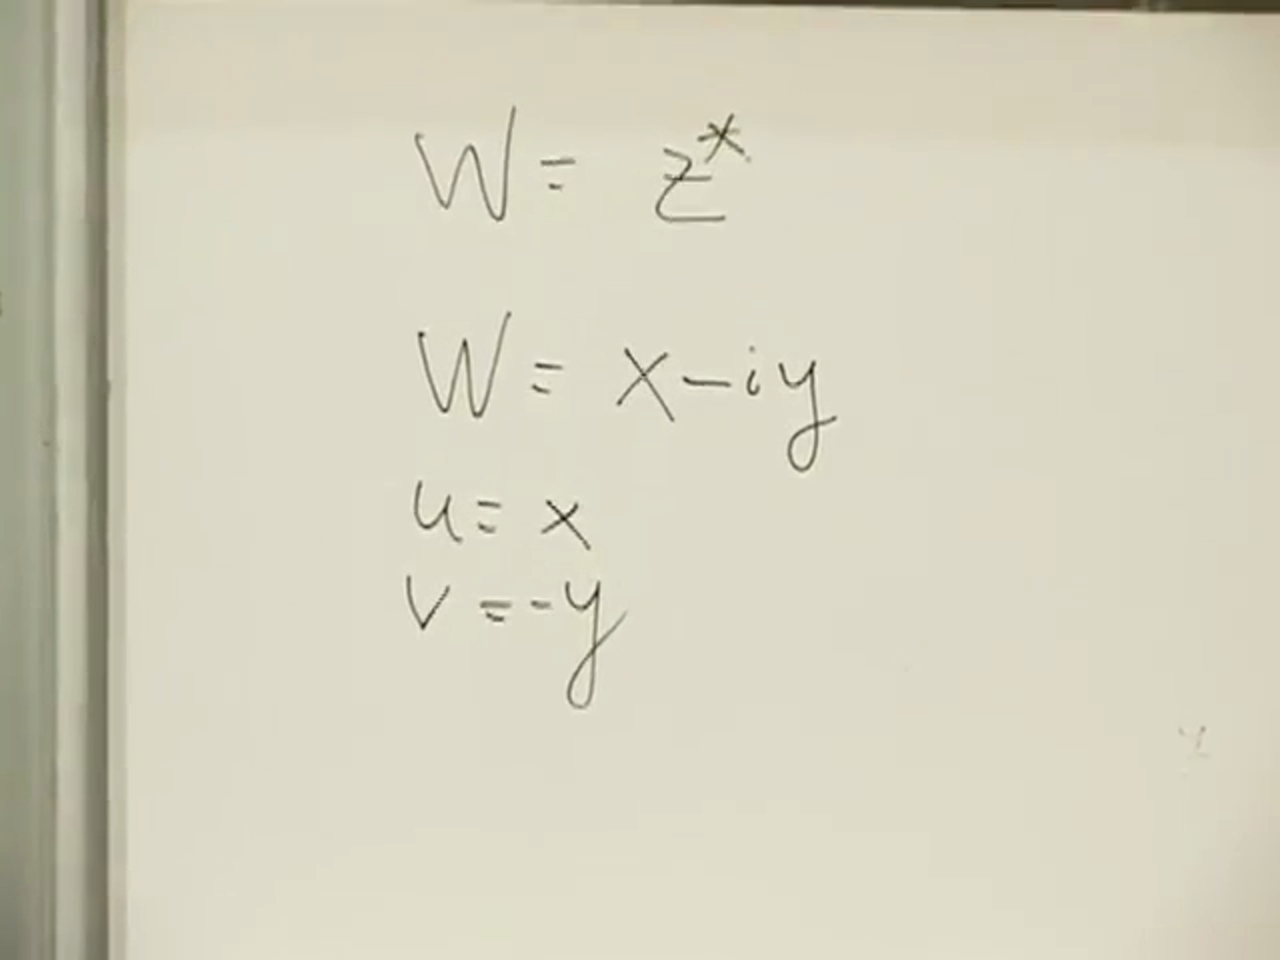
\includegraphics[width=0.62\textwidth]{lecture_08_figure_06.png}
  \caption{複素共役は意図的に非解析的な反例を与える。}
  \lectureframe{00:38:38}
  \label{fig:l08-conjugate-board}
\end{figure}

\subsection{指数関数とその逆関数}

\begin{classroomqa}
\audiencequestion{\(e^z\)が解析的なら、なぜその逆関数\(\log z\)も解析的であるべきか？\lecturetimestamp{00:40:38}}
\lecturerresponse{逆関数が存在し\(w'(z)\neq0\)であるところでは、その導関数は\(1/w'(z)\)である。したがって方向独立性は保たれる。大域的には対数は多価なので、分枝を選び、その分枝点と分枝切断を除外する。局所的な等角の主張はその選ばれた定義域上で依然として有効である。}
\end{classroomqa}

オイラーの公式より
\begin{equation}
  w=e^z=e^{x+iy}
  =e^x(\cos y+i\sin y),
\end{equation}
したがって
\begin{equation}
  u=e^x\cos y,
  \qquad
  v=e^x\sin y.
  \label{eq:l08-exponential-components}
\end{equation}
例えば、\(\partial_xu=e^x\cos y=\partial_yv\)であり、第二のコーシー--リーマンの方程式も同様に直接従う。

\begin{figure}[H]
  \centering
  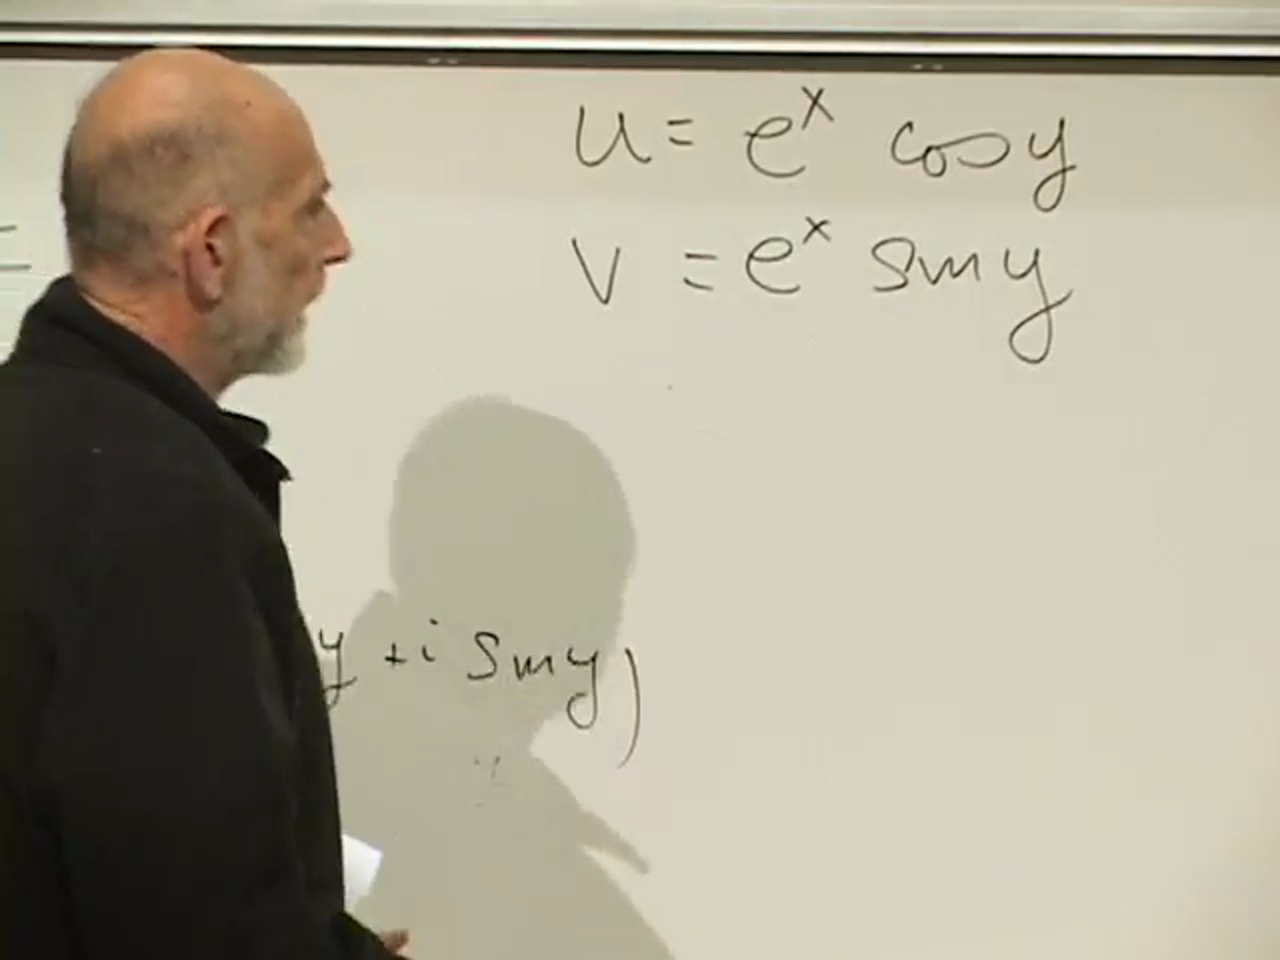
\includegraphics[width=0.68\textwidth]{lecture_08_figure_07.png}
  \caption{指数写像の実部と虚部の成分。}
  \lectureframe{00:42:23}
  \label{fig:l08-exponential-board}
\end{figure}

\section{半平面、帯、円柱、円板}

\subsection{対数は半径を時間に変える}

右半平面をとり、そこでは
\(-\pi/2<\theta<\pi/2\)であり、
\begin{equation}
  z=re^{i\theta},
  \qquad
  w=\log z=\log r+i\theta.
  \label{eq:l08-log-map}
\end{equation}
と書く。半平面は無限帯
\begin{equation}
  -\frac{\pi}{2}<\operatorname{Im}w<\frac{\pi}{2}.
\end{equation}
に写る。\(\theta\)を固定した半直線は水平線になり、\(r\)を固定した半円は垂直線になる。原点は\(\operatorname{Re}w=-\infty\)に送られ、\(r=\infty\)は\(\operatorname{Re}w=+\infty\)に送られる。

\begin{figure}[H]
  \centering
  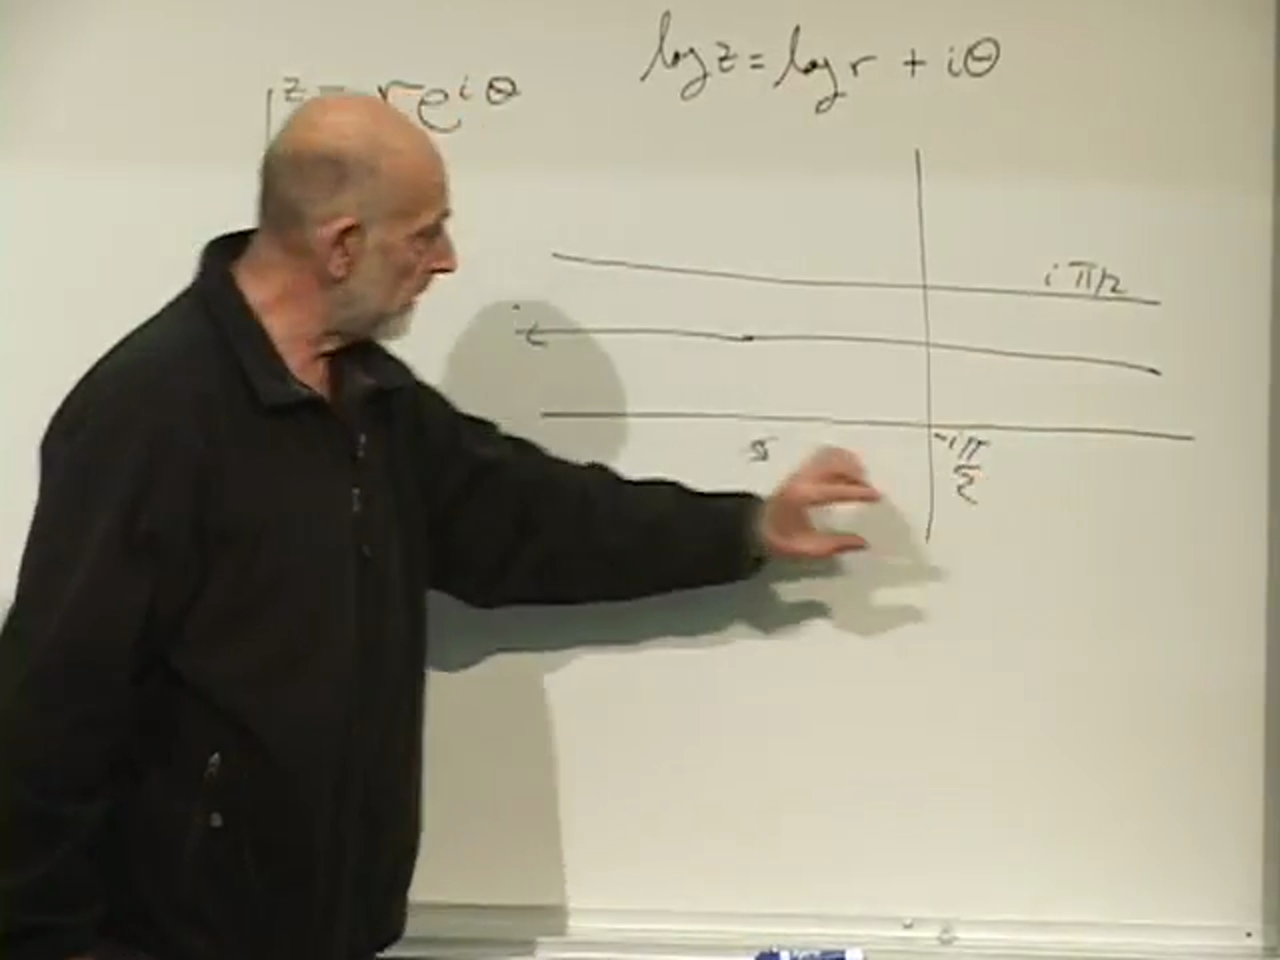
\includegraphics[width=0.75\textwidth]{lecture_08_figure_08.png}
  \caption{対数は右半平面を無限帯に移す：極座標の半直線と半円は直交する長方形格子になる。}
  \lectureframe{00:47:48}
  \label{fig:l08-log-strip-board}
\end{figure}

この帯は開弦の標準的な世界面である。その有界な座標は弦に沿ったパラメータであり、非有界方向に沿った平行移動は世界面時間である。逆指数写像の下で、時間の平行移動は膨張 \(z\mapsto e^a z\) になる。したがって同じ対称性は、帯上では平行移動、半平面上では一様な拡大として見える。

\begin{classroomqa}
\audiencequestion{\(r=1\) のような特定の値はどこへ行くのか、また帯上の座標は依然として極座標なのか。\lecturetimestamp{00:50:58}}
\lecturerresponse{固定された半径の円は \(\operatorname{Re}w=\log r\) における垂直線になる。特に \(r=1\) は中心線 \(\operatorname{Re}w=0\) に写像される。極座標は \(z\) 平面を記述する。\(w\) 平面は通常の直交座標 \((\log r,\theta)\) を用いる。}
\end{classroomqa}

穴あき平面全体が \(\log z\) によって写像されるなら、角度座標の周期は \(2\pi\) である。したがって得られる帯は上端と下端が同一視される。すなわち無限円筒である。境界を持つ半平面は開弦の世界面を記述し、境界がなく角度が周期的な平面全体は閉弦の円筒を記述する。

\begin{figure}[H]
  \centering
  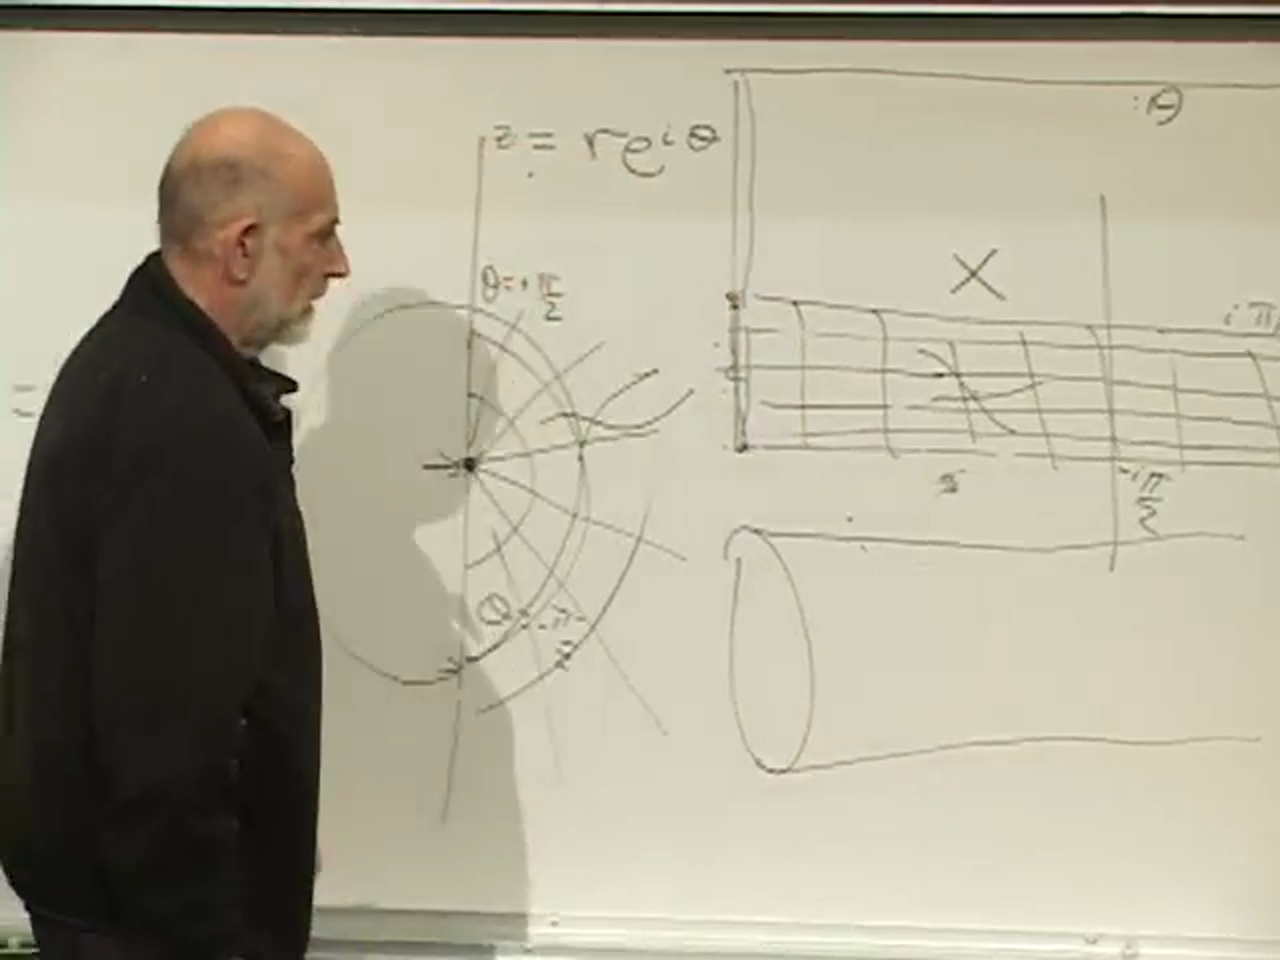
\includegraphics[width=0.75\textwidth]{lecture_08_figure_09.png}
  \caption{半平面／帯の描像と、穴あき平面全体を閉弦の円筒に変える周期的同一視。}
  \lectureframe{00:54:23}
  \label{fig:l08-open-closed-board}
\end{figure}

\subsection{単位円板へのケイリー写像}

線形分数写像、すなわちメビウス写像は右半平面を単位円板へ写す：
\begin{equation}
  w=\frac{z-1}{z+1}.
  \label{eq:l08-cayley}
\end{equation}
これは \(z=0\) を \(-1\) へ、\(z=\infty\) を \(+1\) へ、虚軸を \(|w|=1\) へ写す。\(z=ir\) ならば、
\begin{equation}
  \left|\frac{ir-1}{ir+1}\right|=1.
\end{equation}
\(\operatorname{Re}z>0\) である点は円の内側にあり、左半平面はその外側へ写像される。
\editorialnote{実時間の導出では、円板内部の像を説明しながら逆数 \((z+1)/(z-1)\) が書かれる。その逆数は同じ単位円の境界を持つが、右半平面を外部へ写す。方程式 \eqref{eq:l08-cayley} が、述べられた幾何学と整合する円板内部の規約である。}

\begin{figure}[H]
  \centering
  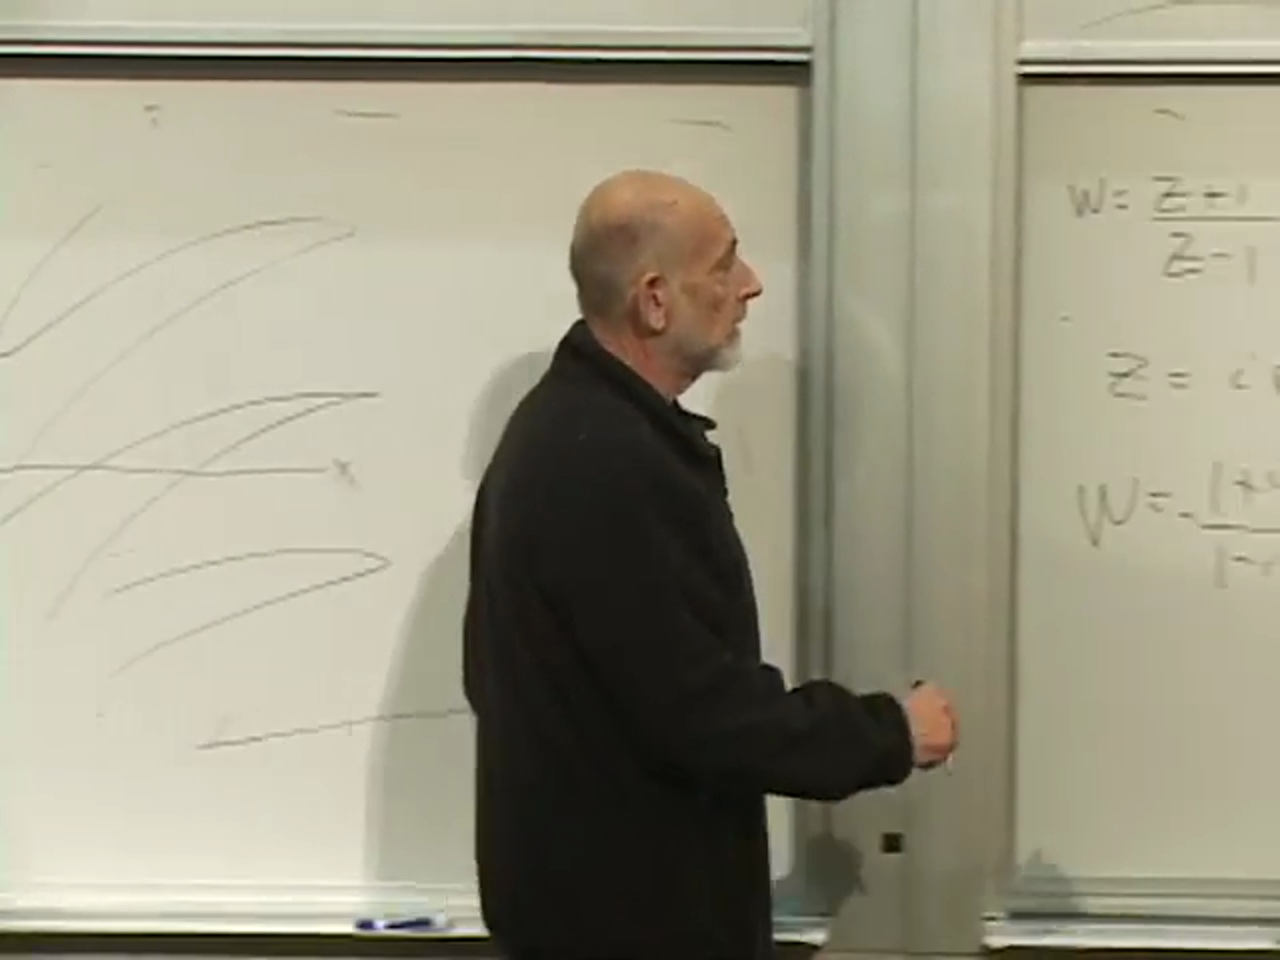
\includegraphics[width=0.72\textwidth]{lecture_08_figure_10.png}
  \caption{単位円境界の線形分数構成。黒板上に見える逆数の規約は内部と外部を交換する。}
  \lectureframe{00:58:38}
  \label{fig:l08-cayley-board}
\end{figure}

メビウス写像は、円と直線の一般化された集まりを円と直線へ写す。したがって半平面上の動径方向と円周方向の格子は、円板上の二つの直交する弧の族になる。直線の直径は、中心が無限遠へ行った円の極限の場合にすぎない。

\begin{classroomqa}
\audiencequestion{円板の内側に描かれた弧は本当に円なのか。\lecturetimestamp{01:00:55}}
\lecturerresponse{はい。それらの中心は異なる位置にあり、しばしば可視の円板の外側にある。直径は同じ族の無限半径極限である。}
\end{classroomqa}

\begin{classroomqa}
\audiencequestion{円板の図はそれが球であることを意味するのか、またもう一方の半平面はどこへ行くのか。\lecturetimestamp{01:01:21}}
\lecturerresponse{ここでの図は平らな円板であり、球ではない。右半平面はその境界の内側へ写像され、左半平面は外側へ写像される。複素平面全体に無限遠点を加えるなら、その拡張平面はステレオ投影によって球として表すことができる。それは別の大域的な主張である。}
\end{classroomqa}

\begin{classroomqa}
\audiencequestion{どの円板内の曲線が、元の動径方向のスポークと一定半径の半円に対応するのか。\lecturetimestamp{01:02:59}}
\lecturerresponse{正の実軸は \(-1\) と \(+1\) を結ぶ直径になる。他の光線は同じ境界点を結ぶ円弧になる。固定された半径の半円は、単位円上で始まり終わる直交する族になる。}
\end{classroomqa}

\begin{figure}[H]
  \centering
  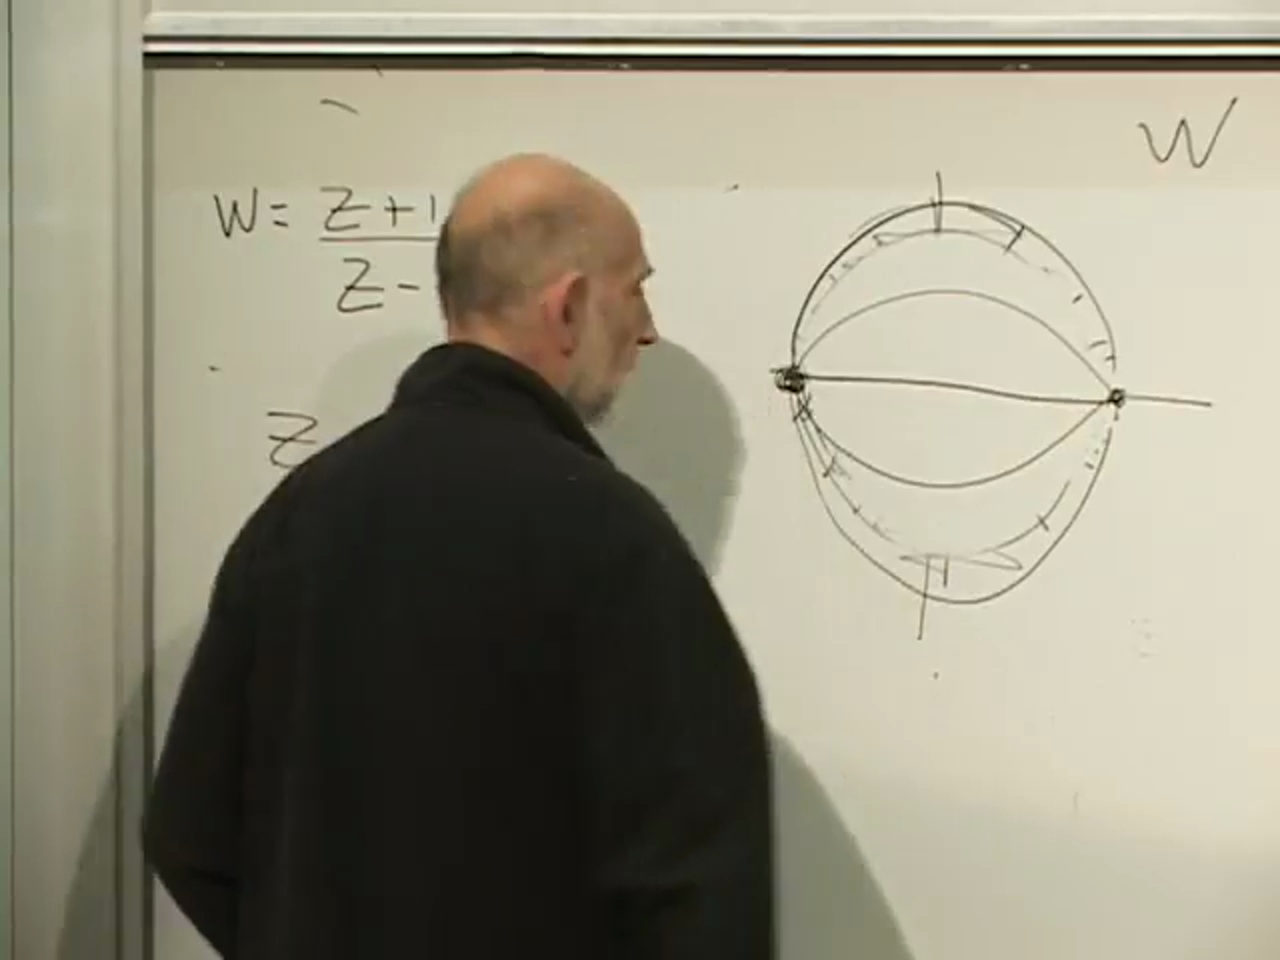
\includegraphics[width=0.72\textwidth]{lecture_08_figure_11.png}
  \caption{半平面内の直線と半円は、円板内の直交する円と直線の族になる。}
  \lectureframe{01:03:48}
  \label{fig:l08-circle-grid-board}
\end{figure}

\section{四本の弦の世界面}

ここで散乱に戻ることができる。二本の開弦が入射し、一本の弦に結合し、任意の区間だけ伝播し、二本の出射弦に分裂する。帯座標では、世界面は両端から切り込まれた長いリボンのように見える---「スポーツ用絆創膏」の描像である。中間の寿命はあらかじめ選ばれていない。それは振幅が積分される履歴の一つである。

\((\sigma,\tau)\) を世界面上の座標とし、\begin{equation}
  X^\mu=X^\mu(\sigma,\tau)
  \label{eq:l08-embedding}
\end{equation} が時空内のその位置を与えるとする。ラベル \(\sigma,\tau\) は二次元パラメータ面上にあり、添字 \(\mu\) は時空座標をラベル付けする。ボソン的理論では \(\mu=0,\ldots,25\) であり、超弦の場合には十個の時空座標がある。

ウィック回転の後、自由埋め込み場は次のユークリッド作用を持つ：
\begin{equation}
  S_E[X]
  =\frac{1}{4\pi\alpha'}\int_\Sigma d\sigma\,d\tau\,
  \left[
    \partial_\tau X^\mu\partial_\tau X_\mu
    +\partial_\sigma X^\mu\partial_\sigma X_\mu
  \right].
  \label{eq:l08-euclidean-action}
\end{equation}
対応する経路積分は、選ばれた世界面の時空へのあらゆる埋め込みにわたって和をとる：
\begin{equation}
  \int\mathcal D X\,e^{-S_E[X]}.
  \label{eq:l08-bare-worldsheet-integral}
\end{equation}

\begin{figure}[H]
  \centering
  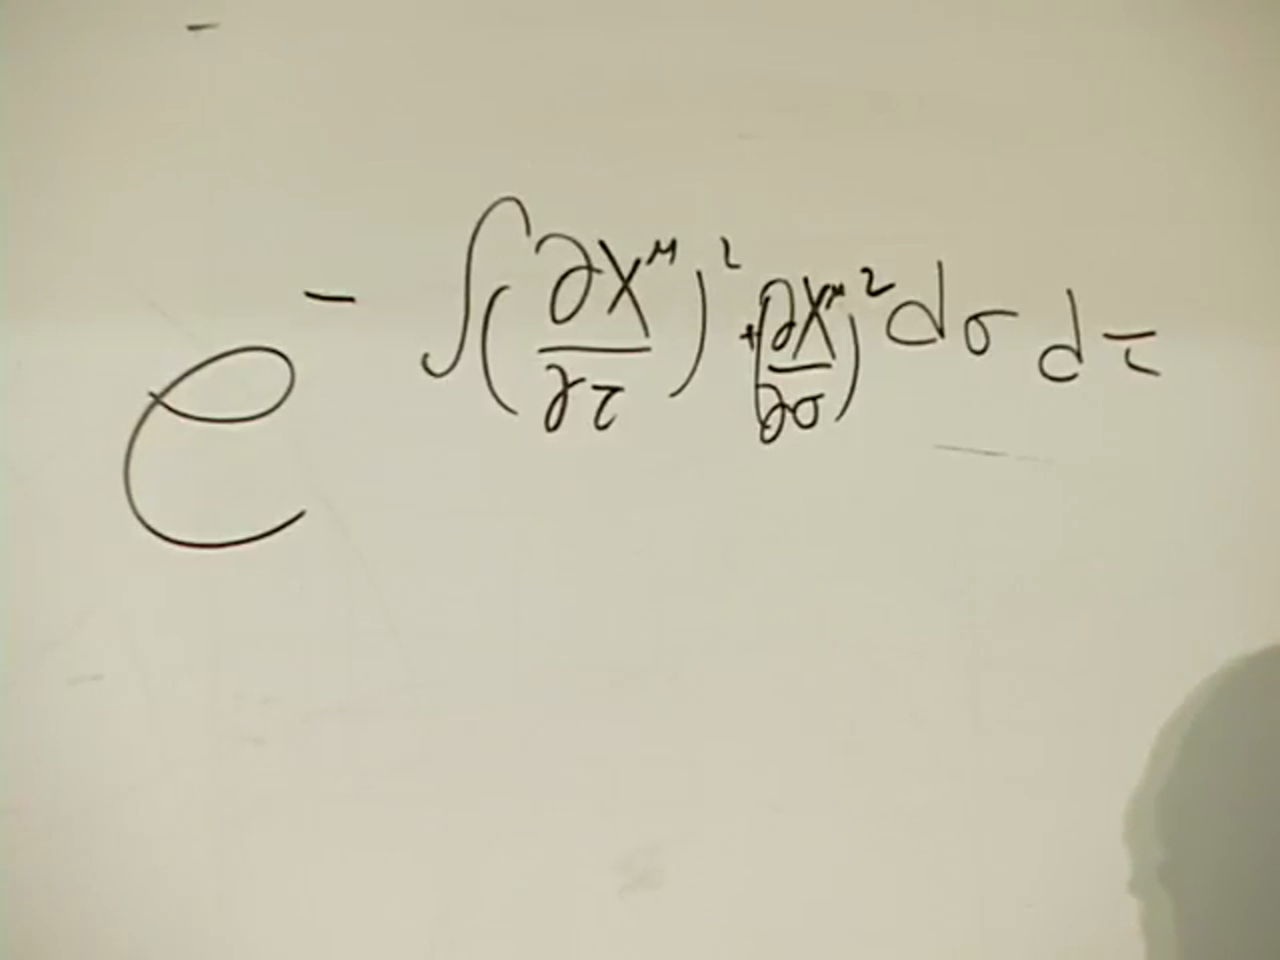
\includegraphics[width=0.74\textwidth]{lecture_08_figure_12.png}
  \caption{完成した正のユークリッド世界面重み。二つの微分項はすべての時空成分にわたって和をとられる。}
  \lectureframe{01:11:34}
  \label{fig:l08-action-board}
\end{figure}

スリットの入った帯は一つの連結した境界を持つ。したがって共形自由度により、それは円板として表すことができる。帯の四つの遠方の端は境界上の四つの印された点となる。印された点を変形すると、帯座標における結合と分裂の間の見かけの分離は変わるが、根底にある曲面や物理は変わらない。

\begin{figure}[H]
  \centering
  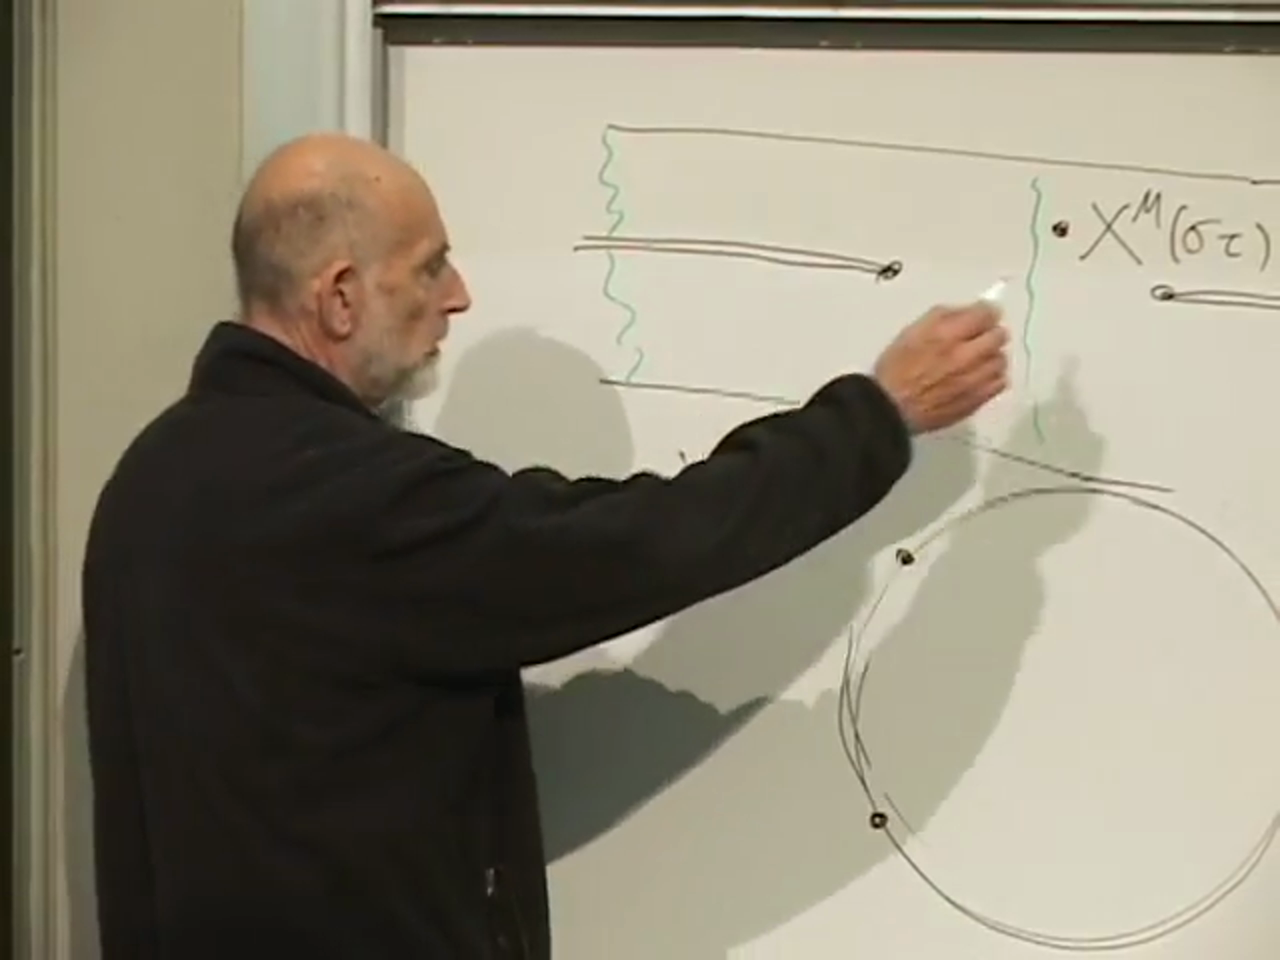
\includegraphics[width=0.76\textwidth]{lecture_08_figure_13.png}
  \caption{スリットの入った帯の世界面と、外部弦に対する境界点を伴うその円板表示。}
  \lectureframe{01:15:18}
  \label{fig:l08-bandage-disc-board}
\end{figure}

この共形写像を描くために用いられる細かな格子線は物理的内容を持たない。重要なのは位相、境界、そして印された外部点である。同じ世界面は、新たな相互作用を導入することなく、異なるチャネルの描像へと引き伸ばすことができる。

\section{境界挿入としての外部状態}

裸の積分\eqref{eq:l08-bare-worldsheet-integral}は、どの運動量が入り、どの運動量が出るかをまだ述べていない。運動量\(k_i^\mu\)のスカラー開弦状態に対しては、境界上に頂点演算子
\begin{equation}
  V_i(z_i)=e^{\,i k_i\cdot X(z_i)},
  \qquad
  k_i\cdot X=k_{i\mu}X^\mu.
  \label{eq:l08-vertex}
\end{equation}
を挿入する。点\(z_i\)は世界面境界上の位置である。それは時空座標ではなく、運動量の方向でもない。

\begin{figure}[H]
  \centering
  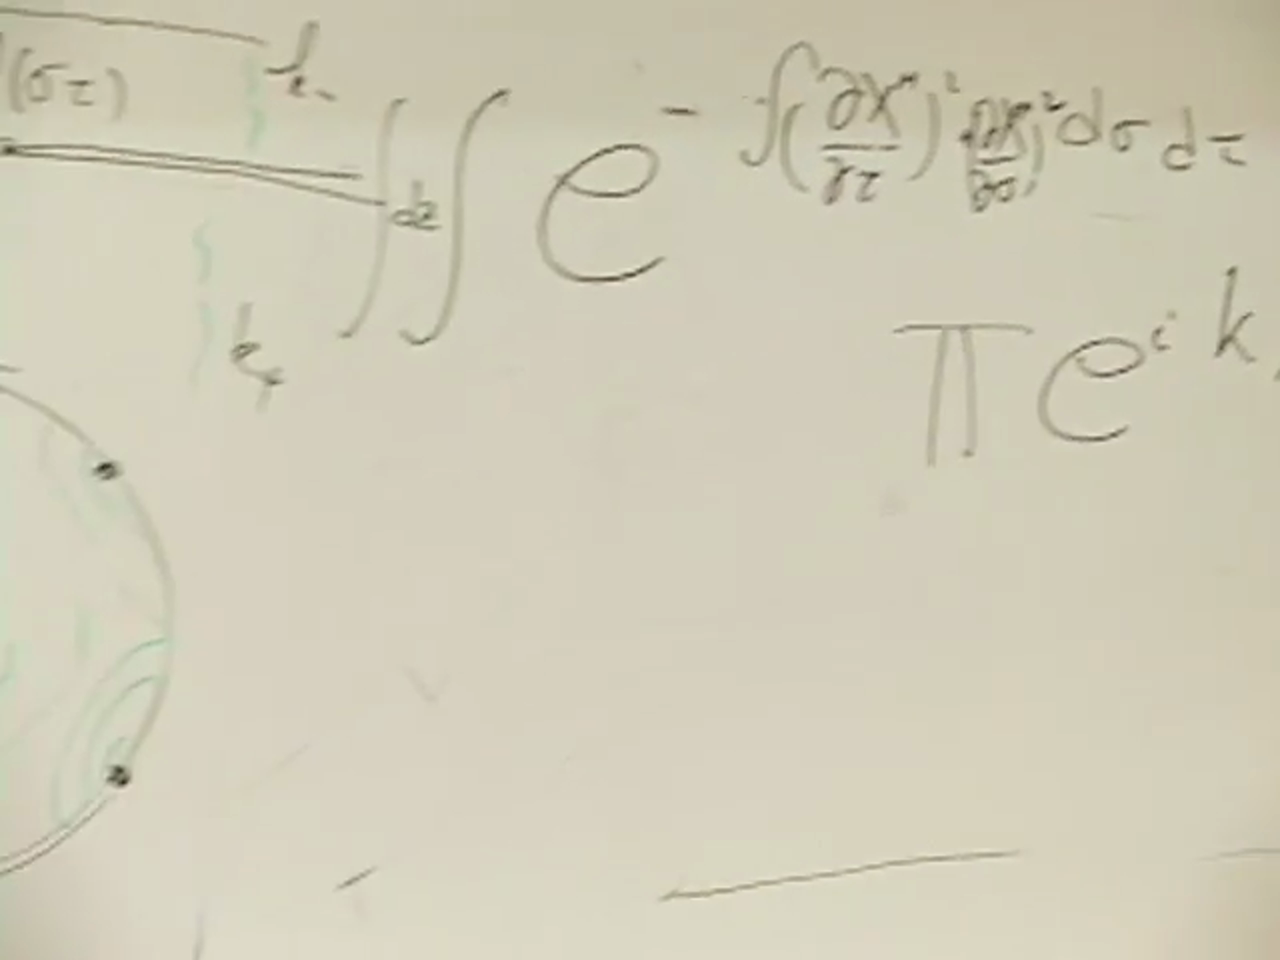
\includegraphics[width=0.72\textwidth]{lecture_08_figure_14.png}
  \caption{バルクのユークリッド重みと境界運動量挿入の積が、別個の因子として表示されている。}
  \lectureframe{01:18:58}
  \label{fig:l08-vertex-board}
\end{figure}

\(n\)個の外部開弦に対して、概略的な処方は
\begin{equation}
  \begin{aligned}
    \mathcal A_n(k_1,\ldots,k_n)
    &=\int_{\mathcal M_{0,n}^{\partial}}\!d\mu(z_i)
      \int\mathcal D X\\
    &\quad\times e^{-S_E[X]}
      \prod_{i=1}^{n}e^{\,i k_i\cdot X(z_i)}.
  \end{aligned}
  \label{eq:l08-open-string-prescription}
\end{equation}
である。関数積分は埋め込み\(X^\mu\)にわたる。有限次元積分は非等価な境界挿入位置にわたる。偏極因子とゲージ固定の測度は、講義におけると同様、この段階では省略されている。
\editorialnote{完全なゲージ固定された弦振幅はまた、適切なゴースト寄与、状態依存の頂点因子、結合定数、規格化を含む。方程式
\eqref{eq:l08-open-string-prescription}は、この講義で展開された埋め込み場と位置の依存性を記録している。}

\begin{classroomqa}
\audiencequestion{外部運動量が固定されているなら、なぜそれらは積分されるのか？\lecturetimestamp{01:20:42}}
\lecturerresponse{積分されない。\(k_i\)は散乱振幅の固定されたラベルである。積分されるのは埋め込み場と、それらの固定された運動量が挿入される世界面上の位置\(z_i\)である。後者の積分は、帯の描像における中間寿命にわたる積分を置き換える。}
\end{classroomqa}

\begin{classroomqa}
\audiencequestion{頂点因子の積は経路積分の内部にあり、作用の一部なのか？\lecturetimestamp{01:21:39}}
\lecturerresponse{それは関数積分の内部で\(e^{-S_E}\)に掛かる。等価に、それらの因子を指数化し、作用に加えられた局所的な源項とみなすこともできるが、概念的にはそれらは自由バルク作用の一部ではなく頂点演算子である。}
\end{classroomqa}

\begin{figure}[H]
  \centering
  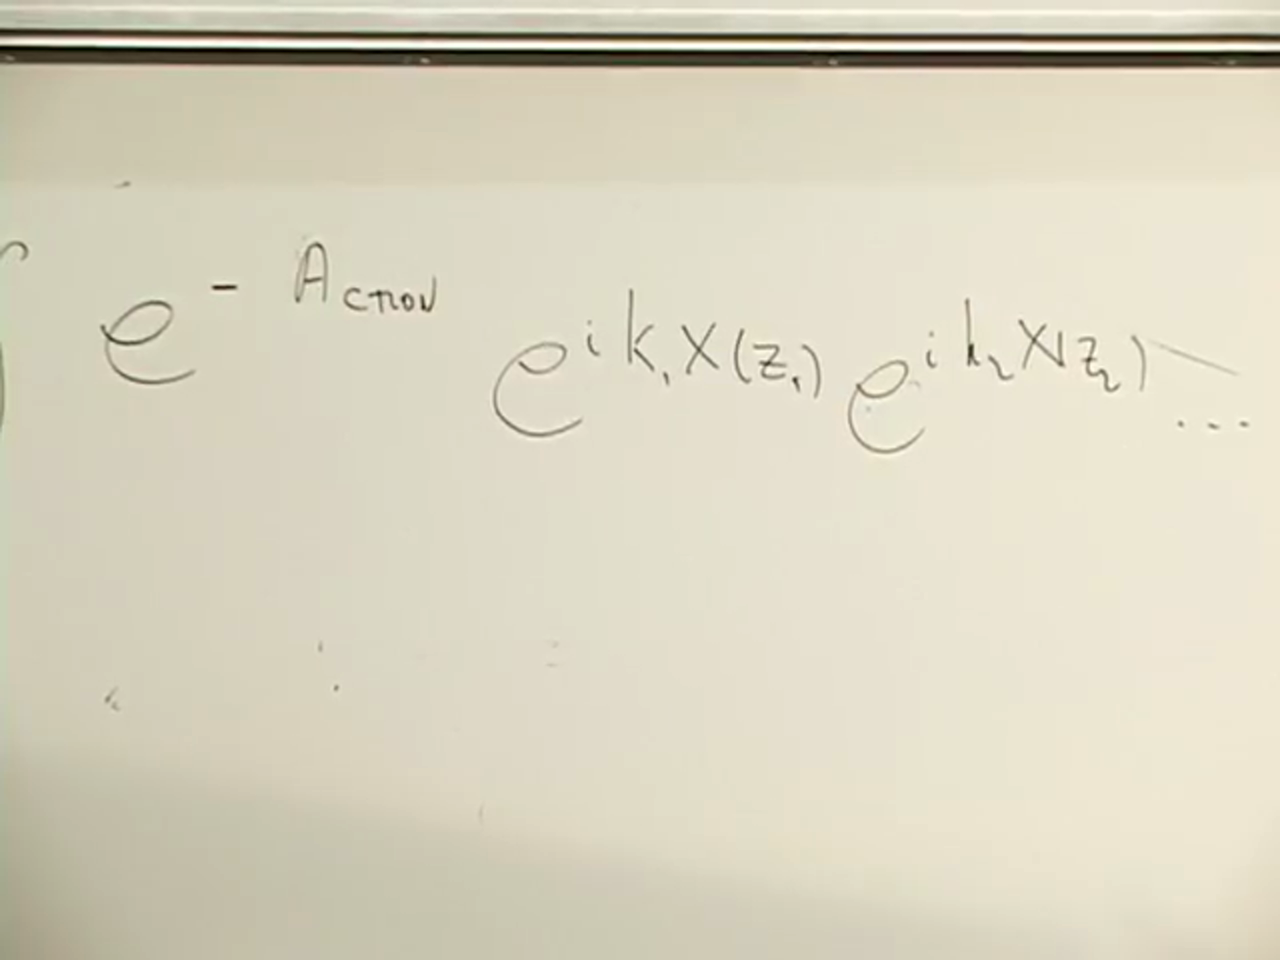
\includegraphics[width=0.76\textwidth]{lecture_08_figure_15.png}
  \caption{連続する外部粒子に対する別個の因子\(e^{ik_i\cdot X(z_i)}\)を用いて書かれた経路積分。}
  \lectureframe{01:23:23}
  \label{fig:l08-full-prescription-board}
\end{figure}

\begin{classroomqa}
\audiencequestion{世界面のウィック回転の後、なぜ\(e^{ik\cdot X}\)は依然として\(i\)を含むのか？\lecturetimestamp{01:23:42}}
\lecturerresponse{回転は世界面の時間を変え、バルク重みを\(e^{iS}\)から\(e^{-S_E}\)へと変換する。運動量固有関数における\(i\)は、時空運動量をラベル付けするフーリエ位相である。それは異なる役割を持ち、残る。}
\end{classroomqa}

\begin{classroomqa}
\audiencequestion{位置\(z_i\)は運動量ベクトルの方向を決定するのか？\lecturetimestamp{01:24:19}}
\lecturerresponse{いいえ。方向は時空成分\(k_i^\mu\)に符号化されている。挿入点\(z_i\)は、その運動量が世界面の記述にどこで入るかを述べる；\(X^\mu(z_i)\)は\(\mathcal D X\)によって和をとられる場の値の一つである。}
\end{classroomqa}

\begin{classroomqa}
\audiencequestion{描かれたバンデージの脚の角度は物理的運動量の方向を符号化しているのか？\lecturetimestamp{01:25:07}}
\lecturerresponse{いいえ。バンデージはパラメータ空間であり、物理的時空における弦の像ではない。その脚は水平に、傾けて、あるいは共形的に曲げて描かれてもよい。物理的方向は成分\(k^\mu\)によって担われ、一方\(X^\mu(\sigma,\tau)\)は積分される。}
\end{classroomqa}

\section{静電学としてのガウス積分}

作用\eqref{eq:l08-euclidean-action}はすべての成分\(X^\mu\)について二次であり、挿入はその指数関数を作用と組み合わせた後では線形な源である。したがって汎関数積分はガウス型である。その鞍点において、各時空成分は模式的に次の形のポアソン方程式を満たす：
\begin{equation}
  \nabla^2 X^\mu(z)
  \propto
  i\alpha'\sum_i k_i^\mu\,\delta(z-z_i),
  \label{eq:l08-electrostatic-source}
\end{equation}
ここで円板の縁には開弦の境界条件が課される。各\(X^\mu\)は独立な静電ポテンシャルのように振る舞い、各運動量成分\(k_i^\mu\)は\(z_i\)に置かれた対応する電荷のように振る舞う。

\begin{figure}[H]
  \centering
  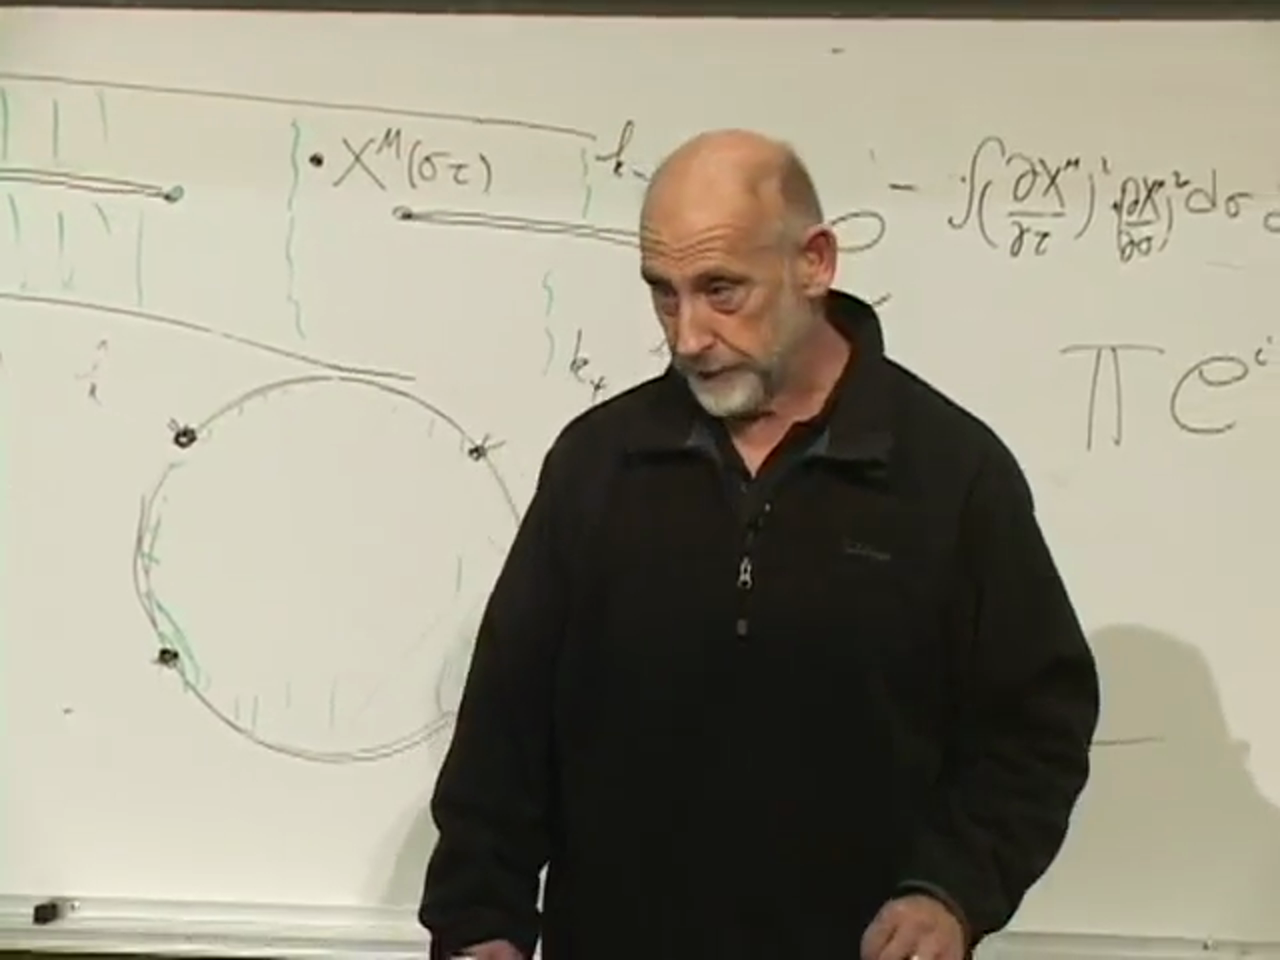
\includegraphics[width=0.76\textwidth]{lecture_08_figure_16.png}
  \caption{境界に源をもつ円板は、各時空成分に対する独立な二次元静電問題として解釈される。}
  \lectureframe{01:28:58}
  \label{fig:l08-electrostatic-disc-board}
\end{figure}

静電問題を解き、そのエネルギーを評価し、負のエネルギーの指数関数をとり、最後に非等価な電荷位置について積分する。標準的な開弦の規格化では、埋め込み場の相関関数がKoba--Nielsen因子を与える：
\begin{equation}
  \left\langle\prod_i e^{\,ik_i\cdot X(z_i)}\right\rangle
  \propto
  (2\pi)^D\delta^{(D)}\!\left(\sum_i k_i\right)
  \prod_{i<j}|z_i-z_j|^{2\alpha' k_i\cdot k_j}.
  \label{eq:l08-koba-nielsen}
\end{equation}
デルタ関数は運動量保存を表す。積は静電対エネルギーを含む。ここで用いた4つのスカラー境界挿入に対して、3つの位置を固定すると、残りの積分は前の講義で現れたEulerベータ積分になる。

\begin{classroomqa}
\audiencequestion{静電エネルギーは26個あるのか、それとも1個だけなのか。\lecturetimestamp{01:30:53}}
\lecturerresponse{各時空成分に対して独立なポテンシャルと場が1つずつある。それらの二次エネルギーは正規直交な標的空間基底では交差項をもたず、寄与は指数関数をとる前に1つの全作用に加えられる。}
\end{classroomqa}

\begin{classroomqa}
\audiencequestion{円板の角度座標は物理的な散乱角なのか。\lecturetimestamp{01:32:10}}
\lecturerresponse{いいえ。それは世界面の位置パラメータである。その非等価な組み合わせは中間伝播区間に関係しており、積分される。物理的な散乱角は、固定された運動量から作られるローレンツ不変量を通して符号化される。}
\end{classroomqa}

\begin{classroomqa}
\audiencequestion{なぜこの構成は臨界次元から離れると失敗するのか。\lecturetimestamp{01:32:35}}
\lecturerresponse{形式的なガウス積分だけが整合性条件のすべてではない。ゲージ固定は共形異常を導入し、その物質とゴーストの寄与は臨界次元でのみ相殺する：ボソン弦では\(D=26\)、超弦では\(D=10\)である。その相殺がなければ、量子世界面の想定された共形対称性は失われる。}
\end{classroomqa}

\begin{classroomqa}
\audiencequestion{すでに3つの大きな空間次元とコンパクトな余剰次元を仮定しているのか。\lecturetimestamp{01:33:38}}
\lecturerresponse{いいえ。コンパクト化はまだこの構成に入っていない。この段階では、ボソン座標は依然として26個すべての標的空間方向にわたり、超弦の場合には10個にわたる。その部分集合がどのように巨視的に大きいままでいられるかが次の議論の主題である。}
\end{classroomqa}

\begin{classroomqa}
\audiencequestion{静電学との関係は、単に座標がラプラス方程式を満たすということだけなのか。\lecturetimestamp{01:33:57}}
\lecturerresponse{そのとおりである。挿入点から離れて、各\(X^\mu\)は調和であり、頂点演算子がデルタ関数の源を与える。静電学の語彙を用いるかどうかにかかわらず、これは点電荷をもつ静的二次元ポテンシャルと同じ数学的境界値問題である。}
\end{classroomqa}

\subsection{共形冗長性とモジュライの数}

円板は3つの実パラメータをもつ共形自己同型群\(\mathrm{PSL}(2,\mathbb R)\)をもつ。したがって3つの順序づけられた境界点を都合のよい位置に固定できる。4本の外部弦に対しては4番目の位置だけが積分に残り、\(n\)個の順序づけられた境界挿入に対しては、ツリーレベルで
\begin{equation}
  n-3
  \label{eq:l08-n-minus-three}
\end{equation}
個の実位置積分がある。

\begin{classroomqa}
\audiencequestion{円板の周りに4つの独立な角度位置があるのか。\lecturetimestamp{01:34:37}}
\lecturerresponse{物理的にはない。最初は4つの位置を書くが、円板の共形対称性により任意の3つを都合のよい場所に置ける。2本入射・2本出射の振幅では、4番目の相対位置だけが残る。}
\end{classroomqa}

\begin{figure}[H]
  \centering
  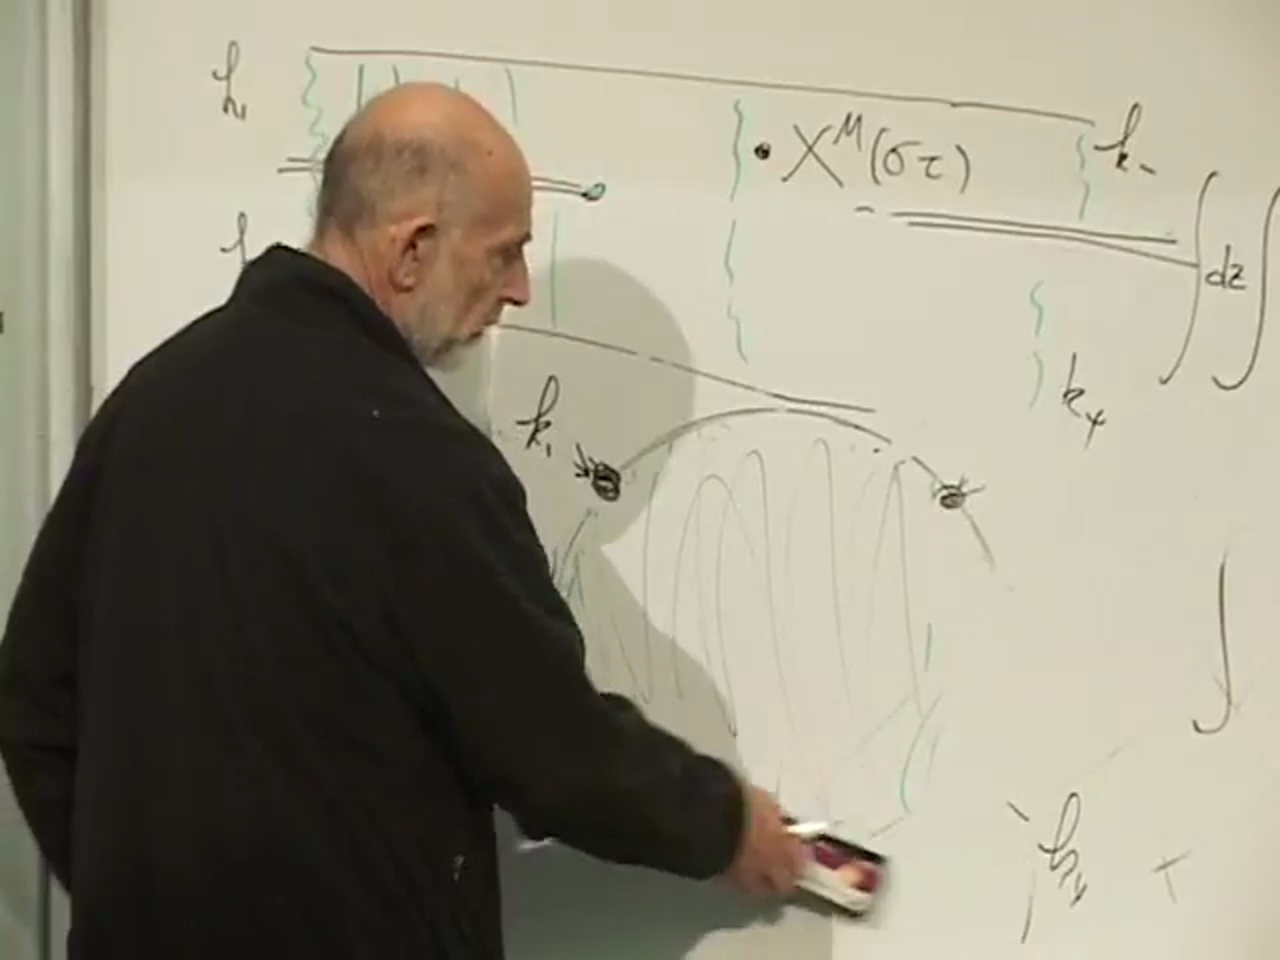
\includegraphics[width=0.72\textwidth]{lecture_08_figure_17.png}
  \caption{円板上の4つの境界挿入。共形自由度は任意の3つを固定し、1つの4点モジュラスを残す。}
  \lectureframe{01:35:18}
  \label{fig:l08-fix-three-board}
\end{figure}

\begin{classroomqa}
\audiencequestion{ストリップ図で2つの分割点が同じ高さにない場合はどうなるのか。\lecturetimestamp{01:35:24}}
\lecturerresponse{共形写像によってその見かけの不一致を移すことができる。異なる図は同じモジュラスの座標代表である。不変な積分は残りの境界位置についての積分であり、等価に伝播区間についての積分である。}
\end{classroomqa}

\begin{classroomqa}
\audiencequestion{より多くの外部粒子がある場合、位置パラメータはいくつ残るか。\lecturetimestamp{01:36:00}}
\lecturerresponse{共形対称性を用いて3つの挿入点を固定し、残りの\(n-3\)を積分する。これが順序付けられたツリーレベルの開弦振幅に対する境界モジュライの数である。}
\end{classroomqa}

\begin{classroomqa}
\audiencequestion{これはM理論とどのように関係するのか。\lecturetimestamp{01:36:37}}
\lecturerresponse{まだ関係しない。ここでの構成はワールドシート上の摂動的な開弦散乱である。そのM理論との関係には後の双対性と非摂動的なアイデアが必要であり、したがってこの問いは明示的に先送りされる。}
\end{classroomqa}

\begin{classroomqa}
\audiencequestion{異なる縦方向または交差したストリップ図は異なる計算なのか。\lecturetimestamp{01:36:49}}
\lecturerresponse{いいえ。都合のよい点を固定し、残りのモジュラスをその全区間にわたって動かせばよい。ストリップ図とディスク上の境界点積分は同じ積分の異なるスライスであり、それゆえすべての外部弦を対称に扱うことができる。}
\end{classroomqa}

\section{この処方箋がまだ解決しないもの}

ディスクの公式は、より多くの外部弦へ直ちに拡張される。より多くの頂点演算子を加え、それらの\(n-3\)個の非等価な境界位置を積分すればよい。これは整合的な弦模型に対する精密なツリーレベルの処方箋であるが、観測される素粒子物理学の現実的な模型ではまだない。単純なボソン的理論は時空次元が誤っており、さらに物理的な欠陥を持つ。超弦はスペクトルを改善し臨界次元を10に下げるが、それでも6つの空間次元をコンパクト化しなければならない。

\begin{classroomqa}
\audiencequestion{この単純な模型はすでに粒子衝突実験と一致するのか。\lecturetimestamp{01:39:06}}
\lecturerresponse{いいえ。共鳴構造は歴史的にはハドロン散乱に似ているが、26次元のボソン的模型は観測される粒子の直接的な記述にはなりえない。この形式論は模型に対する散乱振幅を定義する。自然と一致させるには、現実的なスペクトル、コンパクト化、相互作用、そして真空の選択が必要である。}
\end{classroomqa}

\begin{classroomqa}
\audiencequestion{コンパクト化は余分な次元を減らし、現実的な粒子データを生み出すのか。\lecturetimestamp{01:41:10}}
\lecturerresponse{それは有効な巨視的次元を減らし、粒子スペクトルとゲージ群を生成しうる。また、そこに真の数学的困難の多くが入り込む。多くの整合的なコンパクト化が知られており、観測される素粒子の唯一の模型を選び出すことは未解決のままである。}
\end{classroomqa}

この講義は完成した理論を宣伝するのではなく、この区別を強調する。弦の構成は数学的に明確であり、重力と幾何学について深い情報を生み出してきたが、その多様性それ自体が物理的問題の一部である。

\begin{classroomqa}
\audiencequestion{ボソン的臨界次元が26である理由を短く覚える方法はあるか。\lecturetimestamp{01:43:19}}
\lecturerresponse{以前の振動子計算では正則化された零点和\(1+2+3+\cdots=-1/12\)を用いた。横方向の振動子の寄与は24個の方向を含み、2つの縦方向の時空座標を復元すると\(24+2=26\)となる。これは以前の整合性の議論のための記憶術であり、ここでの新しい導出ではない。}
\end{classroomqa}

\begin{classroomqa}
\audiencequestion{挿入された運動量\(k_i\)自体は量子化されているのか。\lecturetimestamp{01:43:46}}
\lecturerresponse{非コンパクトな時空ではその成分は連続である。量子化されているのは振動子のレベルであり、したがって許される質量二乗スペクトルである。コンパクトな次元は対応する運動量と巻き付きの成分を量子化しうるが、それは次の議論に属する。}
\end{classroomqa}
